\section {SETINGS}

\textit{Settings} tab give us possibility to specify some parameters of application. Parameters are grouped in two section:

\begin{itemize}
	\item Global
	\item Acquisition
\end{itemize}

\subsection{Global}
Section \textit{Global} contains option which allow on change on some settings of application. Description of options is below:
\begin{itemize}
	\item \textit{Start-up language} - select language of application 
	\item \textit{Connection type} - select type of connection with controller of machine
	\item \textit{Chart window} - determine period time of data present on one screen of chart
	\item \textit{Dummy mode} - option generate random data, used to run application when don't have connection with machine controller
\end{itemize}

	\begin{figure}[!h] 
	\centering 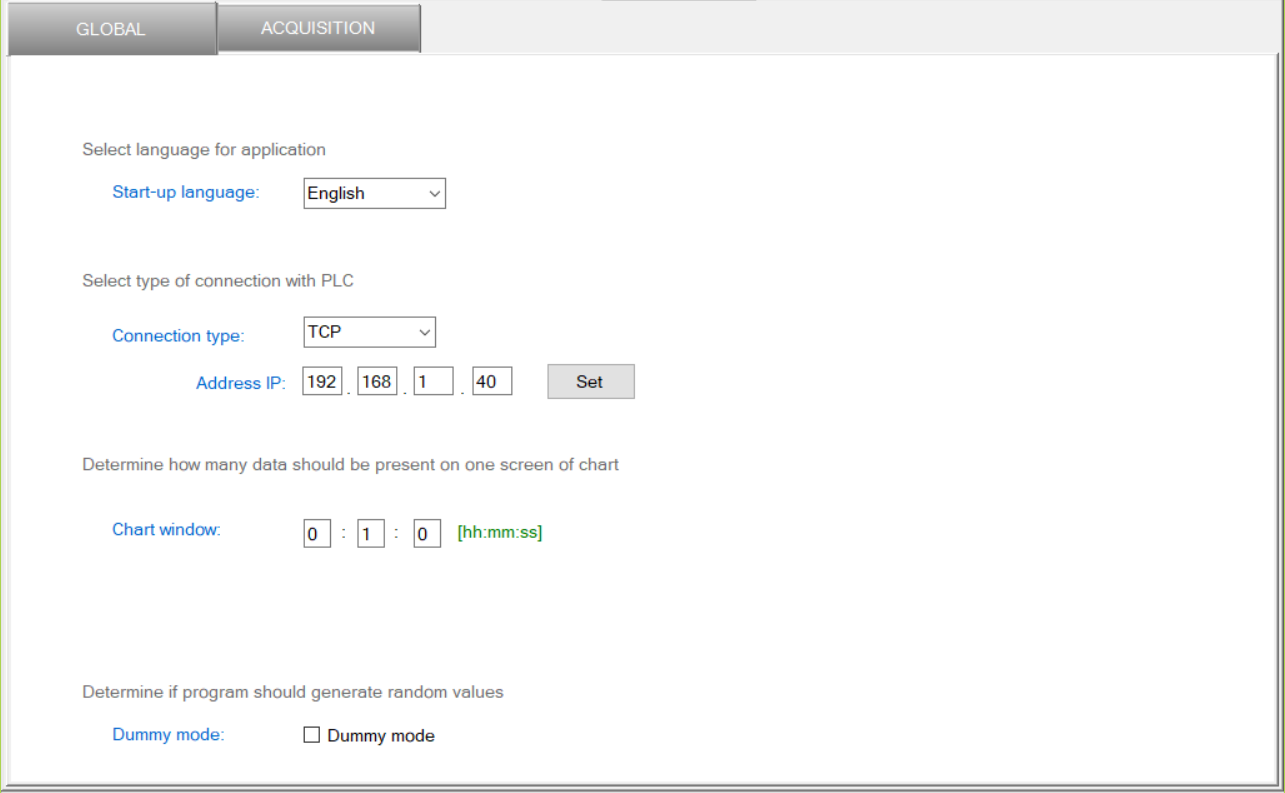
\includegraphics[width=0.8\textwidth]{Graphic/Settings/SettingsGlobal.png}	
	\caption{Settings global options}
	\label{settings_global_options}
	\end{figure}
	\FloatBarrier

\subsection{Acquisition}

\textit{Acquisition} section allow us determine of parameters of archived data process. Options which we can specify are:

\begin{itemize}
	\item \textit{Enabled live acquisition} - determine if data should be automatically saved during executed of automatic  process. When option was disabled any data of process does not saved in archive.
	\item \textit{Enable aks} - determine if we are want to be informed about disabled acquisition data when process is started
	\item \textit{Start acq pressure} - determine level of pressure when data should be saved
	\item \textit{Active option} - option allow enable/disable valid parameter \textit{Start acq pressure.}
	\item \textit {Channels list}
	\begin{itemize}
		\item \textit{Enabled parameter acquisition} - determine If value of channel should be saved in archive
		\item \textit{Frequency} - determine how often data of channel should be saved in archive
		\item \textit{Difference value} - specify level of difference between actual and last value when data of channel should be saved in archive
		\item \textit{Mode} - specify environment when data should be save in archive:according with frequency, according with difference value or mixed both option
	\end{itemize}
\end{itemize} 


	\begin{figure}[!h] 
	\centering 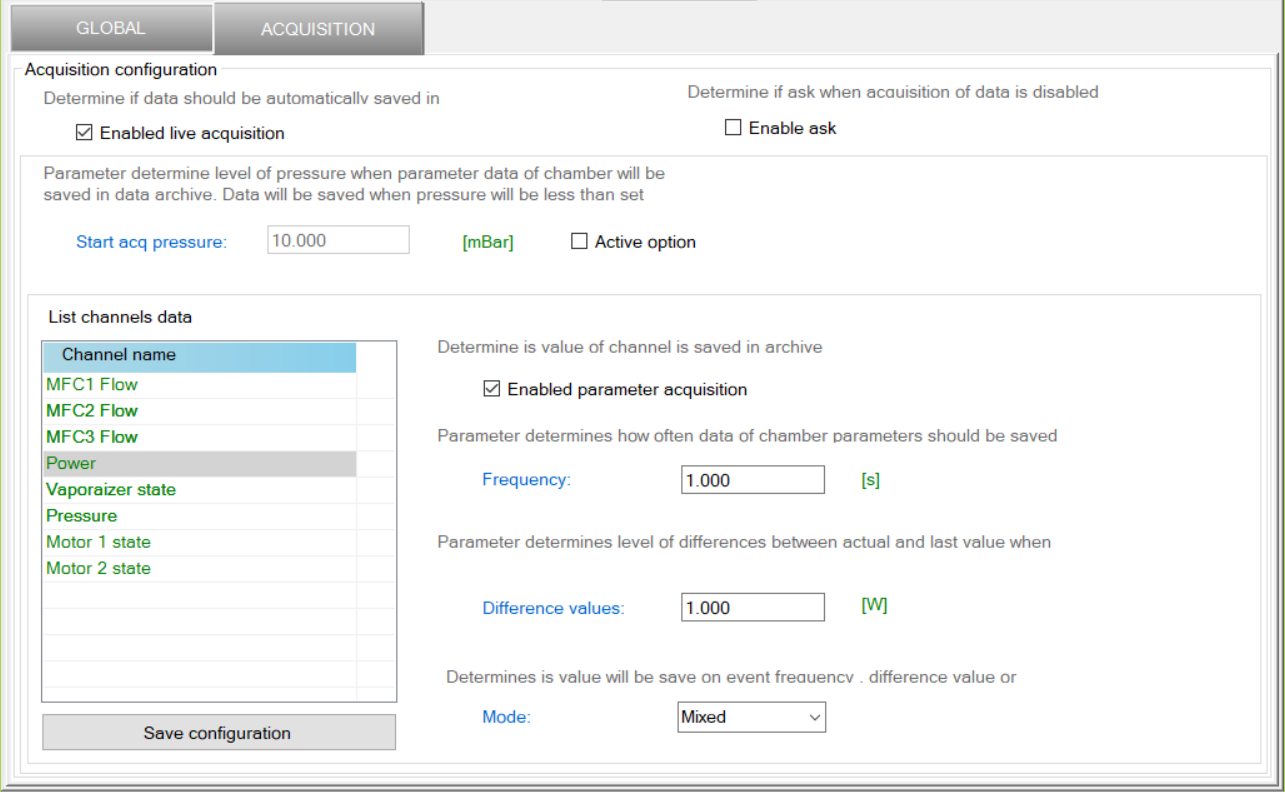
\includegraphics[width=0.8\textwidth]{Graphic/Settings/SettingsAcq.png}	
	\caption{Settings acquisition options}
	\label{settings_acquisition_options}
	\end{figure}
	\FloatBarrier

